\Chapter{Megvalósítás}

\begin{figure}[h]
\centering
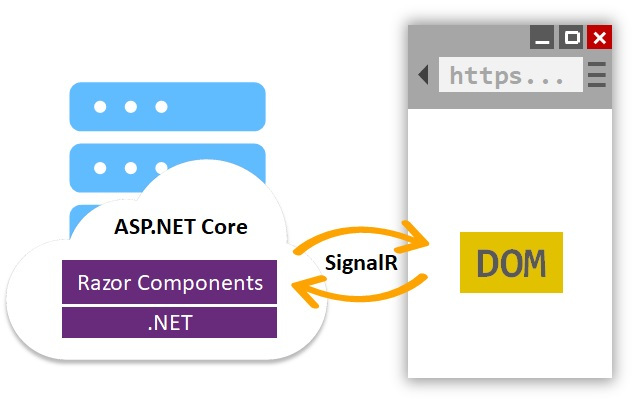
\includegraphics[scale=0.5]{images/blazor.jpg}
\caption{Blazor Server. \\ Forrás:https://docs.microsoft.com/en-us/aspnet/core/blazor/?view=aspnetcore-6.0}
\label{fig:blazor}
\end{figure}

\Section{ASP.NET Core Blazor}
A megvalósításra felhasznált technológia végül a ASP.NET Core Blazor lett, ami egy .Net keretrendszer komplex, interaktív webalkalmazások létrehozására. Lényege, hogy a weboldalhoz  JavaScript helyett C\# kódot írhassunk. Kicsit pontosabban, szinte minden frontend logikához C\# kód a megoldás HTML elemek elrendezésétől a weboldal navigálásán át fájlok feltöltéséig.

Jelenleg 2 verziója támogatott, Blazor Server ahol egy szerver alkalmazásban fut a kód, és Blazor WebAssembly, ahol közvetlenül a böngészőben. Ebben a projektben a Blazor Server-t választottam a nagyobb támogatottsága miatt.

\Section{Razor komponensek}
Blazor alkalmazások jelentős részben Razor komponensekből épülnek fel. Egy komponens az UI egy önálló része, ami tartalmazhat feldolgozó logikát hogy dinamikusan viselkedhessen. Komponenseket lehet többször felhasználni, egymásba ágyazni, vagy Razor oldalakban felhasználni (egy komponens akár önmagában is lehet Razor oldal). Egy Razor komponens tartalmaz HTML elemeket és @ jellel ellátott C\# kifejezéseket, amik lehetnek direktívák, logikák, vagy akár komplex kód részek is.

\Section{Routing, SignalR, and Dependency Injection}
Routing, azaz útvonal választás az a folyamat, ahogy a szerver a bejövő HTTP kéréseket az alkalmazás végrehajtható végpontjaihoz párosítja. Az ASP.Net ezt szinte automatikusan teszi meg, a megfelelő kérést a megfelelő Razor oldalra irányítja, miután megadjuk neki a kellő feltérképezési beállítást. 

Viszont nem minden interakció eredményez HTTP kérést, a legtöbb kommunikáció a weboldal és a szerver között SignalR segítségével történik. A SignalR egy nyílt forrású könyvtár ami lehetővé teszi a valós idejű kommunikációt a szerver és a weboldal között. Ha a UI egy interaktív elemét "megpiszkájuk", a weboldal SignalR-en át átküldi az esemény(eke)t a szervernek, a szerver végrehajtja a kérést, majd szintén SignalR-en keresztül visszaküldi a UI frissítéseket.

A Dependency Injection egy szoftverdizájnbeli minta, aminek lényege, hogy megfordítja az irányítást elemek és függőségeik között. ASP.NET-ben ez annyit jelent, hogy az osztályok vagy komponensek ahelyett hogy önmaguk hoznák létre vagy konstruktorukban kapják meg a függőségeiket, egy úgynevezett DI konténer hozza őket létre. 3 féle módon lehet a függőségeket kezelni:
\begin{itemize}
\item\textbf{Transient Object} Minden esetben új és egyedi objektumot hoz létre.
\item\textbf{Scoped Object} Egy kérésen belül ugyanazt az objektumot biztosítja.
\item\textbf{Singleton Object} Minden esetben ugyanaz a (meglévő) objektum.
\end{itemize}
Ez az alkalmazás főleg Singleton-okat használ szolgáltatások biztosítására és közös adatok elérésére. Mivel végig egy felhasználó dolgozik egy munkamenetben, nincs szükség limitálni a függőségek élettartamát és elérhetőségét.

\Section{Hardware Service}
A .NET Core hivatalosan egy multiplatform alkalmazás, de sajnos még vannak olyan részei amik jelenleg még csak a Windows-t támogatják. A Hardware elemzésére a hivatalosan támogatott módszer a WMI (Windows Management Instrumentation) használata, nevéből adódóan jelenleg csak Windows-on elérhető, ezért más operációs rendszerek esetében az alkalmazás hamis, kitalált adatokkal dolgozik, amíg a Microsoft ki nem terjeszti a támogatását Linuxra és társaira.

\Section{Navigation Menu}
Az alkalmazásban a navigáció különböző oldalak között az oldalsó navigációs menün keresztül történik. Ennek az az érdekessége, hogy a menüpontok csak akkor jelennek meg, ha tartalmuk készen áll. Itt olyan probléma merült fel, hogy a menü nem frissül magától, ezért be kellett iktatni egy új szolgáltatót, a MenuService-t. A MenuService feladata egy esemény kezelése. Ha a programban olyan változás történik ami hatással van a menüre, a szolgáltatás meghívja az eseményt, amit a menü már észlelni tud és lereagálja. 

\Section{Architeture oldal}
Az Architecture oldal fő és egyetlen eleme egy Canvas, pontosabban egy Blazor Extension Canvas, ami azért előnyös mert könnyen manipulálható C\# kóddal. Ez a komponens miután létrehozza a Canvas-t, megrajzolja a Hardware Service által szolgáltatott adatokat, mint a fizikai memória, CPU, GPU. Az egyszerűség kedvéért fix méretű Canvas-al dolgozik, így pixel pontosan meg tudja rajzolni az entitásokat és a kapcsolatokat. A használt eszközöket zöld színnel jelzi.

\Section{Analysis}
Ez az egyik fő alkotóeleme a programnak, itt megvizsgáljuk a beolvasott fájlt, és sorról sorra végigmegyünk rajta OpenCL elemeket kutatva. 

Első lépésben megvizsgálja hogy a program CPU-nak vagy GPU-n fut-e és ez alapján megállapítja a megfelelő Compute Unit mennyiséget, ami processzor esetén a logikai szálakkal egyenértékű. Viszont videokártya esetén ez egy sokkal összetettebb probléma, nem lehet ilyen egyszerűen megmondani a számítási egységek mennyiségét. Például egy Nvidia 1080 videókártyában 2560 shading unit,160 texture mapping unit, és 64 ROP egység található. Ez egyrészt nem látható a WMI számára, másrészt ebből kikövetkezthetetlen a tényleges OpenCL számítási egységek száma. És ettől csak bonyolultabb esetek vannak, lehetnek CUDA magok vagy Tensor magok is, lehet integrált videókártya ami bizonyos erőforrásokon a processzorral osztozik, más gyártású, például AMD videókártyák pedig teljesen más felépítésűek is lehetnek. Ha sikerülne is megállapítani a számítási egységek számát, 3000+ számítási szálat nem lehet jól vizualizálni, ezért videókártya esetén az ábrázolás céljából a program egy kitalált 4 számítási egységgel fog dolgozni.

Második lépésben összegyűjti az OpenCL elemeket egy listában és megadja a hozzájuk tartozó számítási egység számát. Ez lehet:
\begin{itemize}
\item\textbf{0} , ami azt jelenti hogy egy szálon fut szekvenciálisan,
\item\textbf{1,2,3.....} , ami a hozzá tartozó tényleges számítási egység száma,
\item\textbf{-1} , ami azt jelöli hogy az összes elérhető számítási egységen párhuzamosan történik.
\end{itemize}

\Section{Code oldal}
Ez a második megjelenítő felület. 2 egymás mellett lévő konténerből épül fel.
A baloldali konténerben egy dinamikus táblázat foglal helyet ami a már elemzett objektumokat jeleníti meg Gannt diagram formában. A diagram bal oldalán a végrehajtás lépésének indexe, tetején pedig a számítási egységek sorszámai szerepelnek, plusz a 0-s oszlop ami a szekvenciális futást jelzi. A diagram a számítási egységeknek megfelelően az oldal betöltésekor dinamikusan töltődik fel elemekkel. A diagram elemi html gombok, amik tartalmazzák az elemek neveit, valamint a megfelelő funkciókat. Szükséges a ciklusváltozó "elfogása" az ii változó által, ellenkező esetben a függvények mindannyian az alap ciklusváltozó végső értékét fogják használni.

\begin{cpp}
@for(int i = 0; i < Analyzer.myElements.Count; i++)
 {
   int ii = i;
   <tr>
      <td>@(i+1)</td>
      @for(int j = 0; j < Analyzer.CUs+1; j++)
        {
          <td style="min-width:50px">
          @if (j==Analyzer.myElements[ii].ComputeUnit | (j!=0 &
               -1==Analyzer.myElements[ii].ComputeUnit))
             {
                <button title=@Analyzer.myElements[ii].Name @onclick="()
                =>{ChangeColor(Analyzer.myElements[ii].Index);ScrollTo
                Analyzer.myElements[ii].Index);}">@(i+1)</button>
             }
          </td>
        }
   </tr>
 }
\end{cpp}


A második konténerben, vagyis az oldal jobb oldalán magát a forráskódot jelenítjük meg sorokra osztva, az üres sorokat még a feldolgozás közben eltávolítva. Minden sor külön paragrafus elem, id-val ellátva, hogy lehessen rájuk hivatkozni. Itt lesz szerepe a Gannt diagram gombjainak. Egy gomb megnyomásakor a hozzá tartozó elem színe zöldre, a többi pedig fehérre vált. Ez a fent említett SignalR-en keresztül zajlik, majd ugyanitt frissül az oldal és a megfelelő kódsor paragrafusa ténylegesen zöldre vált. Emellett a böngésző a megfelelő helyre is teker, ami JavaScript-et igényel. A program ekkor JavaScript Interop használatával meghív egy JS függvényt ami elvégzi a kérést.

\begin{cpp}
jsRuntime.InvokeAsync<bool>("test","line{" + (i-8) + "}");
\end{cpp}

\Section{Instrukciók és szimulálásuk}
A program az átmeneti kódot instrukció objektumonként kezeli, ami az instrukció típus enumból és különböző adattagokból áll. Az adattagoknak a típusaikon (string, int, double) túl nincs kötött szerepe, hanem az instrukció kezelő szükség szerint használja őket. Az összes adattag nullázható típus, ami szükséges az instrukciók korrekt létrehozásához és működéséhez, viszont bonyolítja kezelésüket.

Az instrukciók 2 féle módon jönnek létre, vagy hamisak és "kitalálja" őket a program a forrásfájl neve alapján, vagy a felhasználó adja meg őket. Az első esetben egy MockInstructionList objektum hozza őket létre, második esetben pedig egy InstructionParser objektum, de egyaránt egy MockInstructionList objektumban lesznek eltárolva egy listában.

\begin{cpp}
public MockInstructionList ParseInstructons(string textInstructions)
        {
            String[] textInstructionArray = textInstructions.Split('|');
            MockInstructionList list = new MockInstructionList();
            foreach(String instruction in textInstructionArray)
            {         
                list._instructions.Add(ParseInstruction(instruction));
            }
            return list;
        }
        
private Instruction ParseInstruction(string textInstruction)
        {
            ......
            return  new Instruction
                (
                    parseInstructionType(instructionType[1]),
                    nullCheck(currentInstructionArray[1]),
                    nullCheck(currentInstructionArray[2]),
                    nullCheck(currentInstructionArray[3]), 
                    nullCheckInt(currentInstructionArray[4]),
                    nullCheckDouble(currentInstructionArray[5]),
                    nullCheckDouble(currentInstructionArray[6]),
                    instructionVar7,
                    instructionVar8
                 );
        }
\end{cpp}


Ezután az instrukciók átkerülnek a DebugService-hez, ahol megtörténik a szimuláció.
Ennek első lépése a változók és tömbök létrehozása és tárolása. Mivel nem lehet előre tudni a változók neveit, típusait, mennyiségeket, dinamikus megoldásra van szükség. Ilyen lehetett volna változó / tömb listák és hozzájuk tartozó szótárak létrehozása. Változó létrehozásakor hozzáadódna listához, majd bekerülne a szótárba mint egy <változó név,index> elempár és a szótáron át lehetne rá hivatkozni. Működőképes, de komplikált és problémás, mivel a szótár egy extra réteg az adatok és az instrukció kezelő között. Minden adattípushoz külön lista - szótár páros lenne szükséges, tömb listák is bonyolítanák.

A megoldás egyszerre bonyolultabb és egyszerűbb. Futásidőben hozunk létre egy osztályt a szükséges adattagokkal. Ehhez felhasználjuk a Reflection könyvtárat, főleg az AssemblyBuilder-t, ModelBuilder-t, és a TypeBuilder-t. Ezek létrehozzák a az osztályt, majd az instrukciók kezelő létrehozza a megfelelő mezőket, amik lehetnek string vagy double változók, vagy tömbök. Az instrukció kezelő az instrukció típusa alapján hívja meg a korrekt metódust. Ekkor egyiknek sincs értéke.

\begin{cpp}
AssemblyBuilder assemblyBuilder = 
AssemblyBuilder.DefineDynamicAssembly(...);
ModuleBuilder moduleBuilder = 
assemblyBuilder.DefineDynamicModule(...);
TypeBuilder typeBuilder = moduleBuilder.DefineType(...);
foreach (Instruction instruction in instructions)
{
        instructionHandler.
        ExecuteDeclaration(instruction, typeBuilder,...);
}


private void CreateType(string name, string type,TypeBuilder typeBuilder)
        {
            switch (type)
            {
                case "string":
                    typeBuilder.DefineField
                    (name,typeof(string),FieldAttributes.Public);
                    break;
                default:
                    typeBuilder.DefineField
                    (name, typeof(double), FieldAttributes.Public);
                    break;
            }
        }
\end{cpp}

Van lehetőség konstruktorokat is megadni és úgy adni értékeket a változóknak, de problémát okozhat ha egy tömb méretét egy változó szabná meg, és a változónak még nincs értéke. Ezért a deklarációk után befejeződik az osztály készítése, és létrejön egy példánya.
Az objektum létrehozása után megkezdődik az igazi szimuláció, az összes instrukció feldolgozásra kerül. Ha hivatkozni szeretnénk egy változóra, az objektumon át érjük el reflekció segítségével, az objektum típusának mezőjének értéket tudjuk így egyszerűen elérni.

\begin{cpp}
private string VarPrint(string name,Object object)
        {
            return "Value of {name} : 
            {object.GetType().GetField(name).GetValue(object)}";
        }
\end{cpp}

Néhány instrukció paramétere lehet érték vagy változó ami értéket tárol. Ilyen esetben az instrukció kezelő dönt.

\begin{cpp}
			double opValue;
            if (doubleValue.HasValue)
            {
                opValue = doubleValue.Value;
            }
            else
            {
                opValue = (double)object.GetType().
                GetField(value).GetValue(object);
            }
\end{cpp}

Érdekesség hogy néha szükséges átváltani az objektum egy double elemét int-é. Ennek módja általában a (int)var -al történik, de az itt hibát okoz a változó ki-be- csomagolása miatt, ezért vagy (int)(double)var -t kell használni, vagy int.convert(var) -t.

Prédikátumok az átmeneti kódban ugrásokra vannak bontva, ha egy prédikátum teljesül, akkor a szimuláció indexe továbbugrik a megjelölt instrukcióhoz. Elöltesztelő ciklus esetén van egy második ugrás a ciklus végén, ami visszaállítja a szimuláció indexét a ciklushoz tartozó prédikátumhoz.

A futtatás során feljegyzésre kerül a instrukció lépésszám, és a a változók és tömbök által lefoglalt memória igény, ami a program minimum memóriaigényének felel meg, valamint méri a futási időt is. 

A szimuláció végig szekvenciálisan fut, mivel a tényleges futási idő különbség elhanyagolható lenne a C\# Task alapú párhuzamos programozási mechanikái miatt. Minden párhuzamos instrukciónak külön Task-ra lenne szüksége, amiket egyesével egy ciklusban kellene szekvenciálisan létrehozni, így nem hogy gyorsítana a szimuláción, de még hátráltatná is.

A szimuláció után a DebugService az ImageService segítségével létrehoz egy szintaxis fát, amin fel van tüntetve az összes instrukció, és a hozzájuk tartozó nyilak. A kép egy dinamikusan bővülő bitmap-ből készül el, így minimális méretű. Itt két érdekesebb probléma merült fel, az egyikben az alkalmazás lementi a készült képet, majd a böngésző megjeleníti. De ha új képre akarunk váltani, a böngésző a régi képet fogja mutatni, mert eltárolta a gyorsítótárban. Így minden kép sorszámot kap, hogy a böngésző észlelje hogy új képre van szükség, és ne a gyorsítótárból szedje elő. 

A másik érdekes probléma a kép dinamikus bővítése közben történt, a képre rárajzolódott minden rendesen, megtörtént az átméretezés, de a tényleges kép a memóriában nem méreteződött át. Olyan mintha a bitmap objektum egyszerre lenne érték és referencia típus, aminek oka ismeretlen. Szerencsére ha explicit módon referencia típusként kezeljük, akkor ez a hiba és gyorsan megoldódik.

\begin{cpp}
public Bitmap AddInstruction(ref Bitmap bitmap,String text,bool jump)
{
      if (bitmap.Width > 220)
      {
           DrawRectangleText(bitmap, text, jump);
           DrawStraightArrow(bitmap);
       }
       else
       {
           DrawRectangleText(bitmap, text, jump);
       }
       bitmap = ResizeBitmap(bitmap, 200);
       return bitmap;
}
\end{cpp}

Miután elkészül a szintaxis fa, az alkalmazás elkészíti a szimuláció oldalt, ahol az eredmények láthatóak.

\Section{Platform függetlenség}
2016-ban megjelent a .Net Core 1.0, ami az addigi .Net keretrendszer platform független verziója lett. A dolgozatban használt .Net 6.0 ennek a legújabb hosszútávú támogatású verziója, ami szintén platform független. A Blazor webalkalmazás szintén platformfüggetlen. Viszont néhány használt könyvtár még nincs  frissítve, ezért Linuxon vagy nem (System.Management - nem használjuk Linuxon), vagy korlátozottan (System.Drawing.Common) működik. Az alkalmazás így is platformfüggetlen, de csak Windowson volt tesztelve.

%\begin{verbatim}
%$ some commands with arguments
%1 2 3 4 5
%$ _
%\end{verbatim}


